% Options for packages loaded elsewhere
\PassOptionsToPackage{unicode}{hyperref}
\PassOptionsToPackage{hyphens}{url}
%
\documentclass[
]{article}
\usepackage{amsmath,amssymb}
\usepackage{lmodern}
\usepackage{ifxetex,ifluatex}
\ifnum 0\ifxetex 1\fi\ifluatex 1\fi=0 % if pdftex
  \usepackage[T1]{fontenc}
  \usepackage[utf8]{inputenc}
  \usepackage{textcomp} % provide euro and other symbols
\else % if luatex or xetex
  \usepackage{unicode-math}
  \defaultfontfeatures{Scale=MatchLowercase}
  \defaultfontfeatures[\rmfamily]{Ligatures=TeX,Scale=1}
\fi
% Use upquote if available, for straight quotes in verbatim environments
\IfFileExists{upquote.sty}{\usepackage{upquote}}{}
\IfFileExists{microtype.sty}{% use microtype if available
  \usepackage[]{microtype}
  \UseMicrotypeSet[protrusion]{basicmath} % disable protrusion for tt fonts
}{}
\makeatletter
\@ifundefined{KOMAClassName}{% if non-KOMA class
  \IfFileExists{parskip.sty}{%
    \usepackage{parskip}
  }{% else
    \setlength{\parindent}{0pt}
    \setlength{\parskip}{6pt plus 2pt minus 1pt}}
}{% if KOMA class
  \KOMAoptions{parskip=half}}
\makeatother
\usepackage{xcolor}
\IfFileExists{xurl.sty}{\usepackage{xurl}}{} % add URL line breaks if available
\IfFileExists{bookmark.sty}{\usepackage{bookmark}}{\usepackage{hyperref}}
\hypersetup{
  pdftitle={Riesgos\_Competitivos},
  hidelinks,
  pdfcreator={LaTeX via pandoc}}
\urlstyle{same} % disable monospaced font for URLs
\usepackage[margin=1in]{geometry}
\usepackage{color}
\usepackage{fancyvrb}
\newcommand{\VerbBar}{|}
\newcommand{\VERB}{\Verb[commandchars=\\\{\}]}
\DefineVerbatimEnvironment{Highlighting}{Verbatim}{commandchars=\\\{\}}
% Add ',fontsize=\small' for more characters per line
\usepackage{framed}
\definecolor{shadecolor}{RGB}{248,248,248}
\newenvironment{Shaded}{\begin{snugshade}}{\end{snugshade}}
\newcommand{\AlertTok}[1]{\textcolor[rgb]{0.94,0.16,0.16}{#1}}
\newcommand{\AnnotationTok}[1]{\textcolor[rgb]{0.56,0.35,0.01}{\textbf{\textit{#1}}}}
\newcommand{\AttributeTok}[1]{\textcolor[rgb]{0.77,0.63,0.00}{#1}}
\newcommand{\BaseNTok}[1]{\textcolor[rgb]{0.00,0.00,0.81}{#1}}
\newcommand{\BuiltInTok}[1]{#1}
\newcommand{\CharTok}[1]{\textcolor[rgb]{0.31,0.60,0.02}{#1}}
\newcommand{\CommentTok}[1]{\textcolor[rgb]{0.56,0.35,0.01}{\textit{#1}}}
\newcommand{\CommentVarTok}[1]{\textcolor[rgb]{0.56,0.35,0.01}{\textbf{\textit{#1}}}}
\newcommand{\ConstantTok}[1]{\textcolor[rgb]{0.00,0.00,0.00}{#1}}
\newcommand{\ControlFlowTok}[1]{\textcolor[rgb]{0.13,0.29,0.53}{\textbf{#1}}}
\newcommand{\DataTypeTok}[1]{\textcolor[rgb]{0.13,0.29,0.53}{#1}}
\newcommand{\DecValTok}[1]{\textcolor[rgb]{0.00,0.00,0.81}{#1}}
\newcommand{\DocumentationTok}[1]{\textcolor[rgb]{0.56,0.35,0.01}{\textbf{\textit{#1}}}}
\newcommand{\ErrorTok}[1]{\textcolor[rgb]{0.64,0.00,0.00}{\textbf{#1}}}
\newcommand{\ExtensionTok}[1]{#1}
\newcommand{\FloatTok}[1]{\textcolor[rgb]{0.00,0.00,0.81}{#1}}
\newcommand{\FunctionTok}[1]{\textcolor[rgb]{0.00,0.00,0.00}{#1}}
\newcommand{\ImportTok}[1]{#1}
\newcommand{\InformationTok}[1]{\textcolor[rgb]{0.56,0.35,0.01}{\textbf{\textit{#1}}}}
\newcommand{\KeywordTok}[1]{\textcolor[rgb]{0.13,0.29,0.53}{\textbf{#1}}}
\newcommand{\NormalTok}[1]{#1}
\newcommand{\OperatorTok}[1]{\textcolor[rgb]{0.81,0.36,0.00}{\textbf{#1}}}
\newcommand{\OtherTok}[1]{\textcolor[rgb]{0.56,0.35,0.01}{#1}}
\newcommand{\PreprocessorTok}[1]{\textcolor[rgb]{0.56,0.35,0.01}{\textit{#1}}}
\newcommand{\RegionMarkerTok}[1]{#1}
\newcommand{\SpecialCharTok}[1]{\textcolor[rgb]{0.00,0.00,0.00}{#1}}
\newcommand{\SpecialStringTok}[1]{\textcolor[rgb]{0.31,0.60,0.02}{#1}}
\newcommand{\StringTok}[1]{\textcolor[rgb]{0.31,0.60,0.02}{#1}}
\newcommand{\VariableTok}[1]{\textcolor[rgb]{0.00,0.00,0.00}{#1}}
\newcommand{\VerbatimStringTok}[1]{\textcolor[rgb]{0.31,0.60,0.02}{#1}}
\newcommand{\WarningTok}[1]{\textcolor[rgb]{0.56,0.35,0.01}{\textbf{\textit{#1}}}}
\usepackage{graphicx}
\makeatletter
\def\maxwidth{\ifdim\Gin@nat@width>\linewidth\linewidth\else\Gin@nat@width\fi}
\def\maxheight{\ifdim\Gin@nat@height>\textheight\textheight\else\Gin@nat@height\fi}
\makeatother
% Scale images if necessary, so that they will not overflow the page
% margins by default, and it is still possible to overwrite the defaults
% using explicit options in \includegraphics[width, height, ...]{}
\setkeys{Gin}{width=\maxwidth,height=\maxheight,keepaspectratio}
% Set default figure placement to htbp
\makeatletter
\def\fps@figure{htbp}
\makeatother
\setlength{\emergencystretch}{3em} % prevent overfull lines
\providecommand{\tightlist}{%
  \setlength{\itemsep}{0pt}\setlength{\parskip}{0pt}}
\setcounter{secnumdepth}{-\maxdimen} % remove section numbering
\ifluatex
  \usepackage{selnolig}  % disable illegal ligatures
\fi

\title{Riesgos\_Competitivos}
\author{}
\date{\vspace{-2.5em}}

\begin{document}
\maketitle

\hypertarget{introducciuxf3n-y-preeliminares-descripciuxf3n-de-la-base-elegida}{%
\section{Introducción y preeliminares: Descripción de la base
elegida}\label{introducciuxf3n-y-preeliminares-descripciuxf3n-de-la-base-elegida}}

En este trabajo, abordamos el análisis de supervivencia de riesgos
competitivos, por lo que el esquema de trabajo cambia un poco respecto
al visto en clase, que es realizar el modelo de Cox. Así mismo, como
tenemos otro enfoque (Al tratar ahora desde el punto de vista de riesgos
competitivos), no aplican las estimaciones de Kaplan-Meier, sino otros
estimadores.

Trabajaremos con la base sir.adm; dispinible en el paquete ``mvna'',
llamado así por las iniciales de ``Multivariate Nelson-Aalen
estimator'', que permite estimar de manera no paramétrica los riesgos
acumulados de transición de modelos de Markov multi-estados arbitrarios,
usando dicho estimador.

\begin{Shaded}
\begin{Highlighting}[]
\FunctionTok{library}\NormalTok{(mvna) }\CommentTok{\#Estimadores de Nelson{-}Aalen}
\end{Highlighting}
\end{Shaded}

\begin{verbatim}
## Warning: package 'mvna' was built under R version 4.1.2
\end{verbatim}

\begin{Shaded}
\begin{Highlighting}[]
\FunctionTok{library}\NormalTok{(lattice) }\CommentTok{\#Apoyo gráfico}
\end{Highlighting}
\end{Shaded}

\begin{verbatim}
## Warning: package 'lattice' was built under R version 4.1.2
\end{verbatim}

\begin{Shaded}
\begin{Highlighting}[]
\FunctionTok{library}\NormalTok{(cmprsk) }\CommentTok{\#Paquetería enfocada a análisis de subdistribución de riesgos competitivos}
\end{Highlighting}
\end{Shaded}

\begin{verbatim}
## Warning: package 'cmprsk' was built under R version 4.1.2
\end{verbatim}

\begin{verbatim}
## Loading required package: survival
\end{verbatim}

\begin{Shaded}
\begin{Highlighting}[]
\FunctionTok{library}\NormalTok{(etm) }\CommentTok{\#Paquetería que nos permite estimar la matriz de transiciones de probabilidad para modelos multiestado de tiempo no homogéneo de espacio finito, usando el estimador Aalen{-}Johansen}
\end{Highlighting}
\end{Shaded}

\begin{verbatim}
## Warning: package 'etm' was built under R version 4.1.2
\end{verbatim}

Cargamos la base de datos

\begin{Shaded}
\begin{Highlighting}[]
\FunctionTok{data}\NormalTok{(sir.adm)}
\end{Highlighting}
\end{Shaded}

Veamos las primeras 5 observaciones

\begin{Shaded}
\begin{Highlighting}[]
\FunctionTok{head}\NormalTok{(sir.adm)}
\end{Highlighting}
\end{Shaded}

\begin{verbatim}
##     id pneu status time      age sex
## 1   41    0      1    4 75.34153   F
## 2  395    0      1   24 19.17380   M
## 3  710    1      1   37 61.56568   M
## 4 3138    0      1    8 57.88038   F
## 5 3154    0      1    3 39.00639   M
## 6 3178    0      1   24 70.27762   M
\end{verbatim}

El datasetcontiene una submuestra aleatoria de 747 pacientes y 6
variables:

id: Es un id generado aleatoriamente para cada paciente

pneu: Es un indicador de si el paciente presentaba neumonía (1) o no la
presentaba (0) al momento de ser admitido en el estudio

status: Un indicador del estatus de la observación: 0 es una observación
censurada, 1 es que el paciente fue dado de alta, 2 es que el paciente
murió

time: Es el tiempo en días

age: La edad del paciente cuando entró al estudio

sex: F para mujer, M para hombre.

\begin{Shaded}
\begin{Highlighting}[]
\FunctionTok{sum}\NormalTok{(}\FunctionTok{is.na.data.frame}\NormalTok{(sir.adm))}
\end{Highlighting}
\end{Shaded}

\begin{verbatim}
## [1] 0
\end{verbatim}

Vemos que no hay ningún dato faltante (NA) en el dataset.

Estas 747 pacientes son de SIR 3 (Spread of nosocomial Infections and
Resistant pathogens, es decir, Esparcimiento de infecciones nosocomiales
y patógenos resistentes), un estudio conjunto en el hospital Charité de
la Universidad de Berlin, Alemania, con una valoración prospectiva de
datos para examinar el efecto de infecciones adquiridad en el hospital,
en terapia-intesiva.

Notemos que se presenta una censura por la derecha.

El dataset contiene información en el estado de admisión de neumonía,
tiempo de estadía en la unidad de terapia intensiva y ``desenlace o
resultado del tratamiento en unidad intensiva'', es decir, si se le dio
de alta al paciente o este murió.

La neumonía es una infección severa, de la cual se tiene la sospecha,
causa el requerimiento de cuidados adicionales (Es decir, una prolongada
estadía en unidades de cuidado intensivo) y de incrementar la
mortalidad.

\begin{Shaded}
\begin{Highlighting}[]
\FunctionTok{sum}\NormalTok{(sir.adm}\SpecialCharTok{$}\NormalTok{status}\SpecialCharTok{==}\DecValTok{0}\NormalTok{)}
\end{Highlighting}
\end{Shaded}

\begin{verbatim}
## [1] 14
\end{verbatim}

14 Observaciones censuradas, es decir, que seguían en unidad intensiva
al final del estudio.

\begin{Shaded}
\begin{Highlighting}[]
\FunctionTok{sum}\NormalTok{(sir.adm}\SpecialCharTok{$}\NormalTok{status}\SpecialCharTok{==}\DecValTok{1}\NormalTok{)}
\end{Highlighting}
\end{Shaded}

\begin{verbatim}
## [1] 657
\end{verbatim}

657 Pacientes que fueron dados de alta

\begin{Shaded}
\begin{Highlighting}[]
\FunctionTok{sum}\NormalTok{(sir.adm}\SpecialCharTok{$}\NormalTok{status}\SpecialCharTok{==}\DecValTok{2}\NormalTok{)}
\end{Highlighting}
\end{Shaded}

\begin{verbatim}
## [1] 76
\end{verbatim}

76 pacientes fallecieron

\begin{Shaded}
\begin{Highlighting}[]
\FunctionTok{sum}\NormalTok{(sir.adm}\SpecialCharTok{$}\NormalTok{status}\SpecialCharTok{==}\DecValTok{2} \SpecialCharTok{\&}\NormalTok{ sir.adm}\SpecialCharTok{$}\NormalTok{pneu}\SpecialCharTok{==}\DecValTok{1}\NormalTok{)}
\end{Highlighting}
\end{Shaded}

\begin{verbatim}
## [1] 21
\end{verbatim}

21 de los pacientes que murieron tenían neumonía al momento de ser
admitidos.

\begin{Shaded}
\begin{Highlighting}[]
\FunctionTok{sum}\NormalTok{(sir.adm}\SpecialCharTok{$}\NormalTok{status}\SpecialCharTok{==}\DecValTok{2} \SpecialCharTok{\&}\NormalTok{ sir.adm}\SpecialCharTok{$}\NormalTok{pneu}\SpecialCharTok{==}\DecValTok{0}\NormalTok{)}
\end{Highlighting}
\end{Shaded}

\begin{verbatim}
## [1] 55
\end{verbatim}

55 de los pacientes que murieron, no tenían neumonía al momento de ser
admitidos

Esta base la elegimos porque nos parece un buen ejemplo de riesgos
competitvos por lo siguiente:

Se investiga el tiempo hasta el final de la estadía y el estatus de el
estado final: Si se dio de alta o murió en el hospital. Un desafío en el
análisis de este dataset es que se ha encontrado que la neumonía
incrementa la probabilidad de morir en el hospital, pero parece no tener
efecto en el \emph{riesgo} de muerte, es decir, no tiene efecto en la
probabilidad diaria de morir en el hospital, dado que uno sigue vivo y
en la unidad de cuidados intensivos al inicio del día.

Los puntos finales competitivos son el ser dado de alta y morir en la
unidad de terapia intensiva

\hypertarget{anuxe1lisis-descriptivo-y-enfoque-no-paramuxe9trico}{%
\section{Análisis descriptivo y enfoque no
paramétrico}\label{anuxe1lisis-descriptivo-y-enfoque-no-paramuxe9trico}}

\hypertarget{funciuxf3n-de-riesgos-acumulados}{%
\subsection{Función de riesgos
acumulados}\label{funciuxf3n-de-riesgos-acumulados}}

Necesitamos modificar primero el dataset en un dataset de tipo
multiestado. Además, renombramos los datos para que, el evento de
interés que es la muerte, corresponda al estado 1, y el estado 2 el
evento competitivo:

\begin{Shaded}
\begin{Highlighting}[]
\CommentTok{\#Transformamos sir.adm a un dataset de tipo multiestado}
\NormalTok{to }\OtherTok{\textless{}{-}} \FunctionTok{ifelse}\NormalTok{(sir.adm}\SpecialCharTok{$}\NormalTok{status }\SpecialCharTok{==} \DecValTok{0}\NormalTok{, }\StringTok{"cens"}\NormalTok{, }\FunctionTok{ifelse}\NormalTok{(sir.adm}\SpecialCharTok{$}\NormalTok{status }\SpecialCharTok{==} \DecValTok{1}\NormalTok{, }\DecValTok{2}\NormalTok{, }\DecValTok{1}\NormalTok{))}
\NormalTok{my.sir.data }\OtherTok{\textless{}{-}} \FunctionTok{data.frame}\NormalTok{(}\AttributeTok{id =}\NormalTok{ sir.adm}\SpecialCharTok{$}\NormalTok{id, }\AttributeTok{from =} \DecValTok{0}\NormalTok{, to, }\AttributeTok{time =}\NormalTok{ sir.adm}\SpecialCharTok{$}\NormalTok{time, }\AttributeTok{pneu =}\NormalTok{ sir.adm}\SpecialCharTok{$}\NormalTok{pneu)}
\end{Highlighting}
\end{Shaded}

Notemos que my.sir.data tiene un componente pneu con el estatus de
neumonía al momento de admisión. Revisamos que hicimos bien el
remombramiento:

\begin{Shaded}
\begin{Highlighting}[]
\FunctionTok{table}\NormalTok{(my.sir.data}\SpecialCharTok{$}\NormalTok{to)}
\end{Highlighting}
\end{Shaded}

\begin{verbatim}
## 
##    1    2 cens 
##   76  657   14
\end{verbatim}

Lo hicimos de manera correcta.

Antes de continuar, necesitamos describir el modelo de riesgos
competitivos muliestado siguiente:

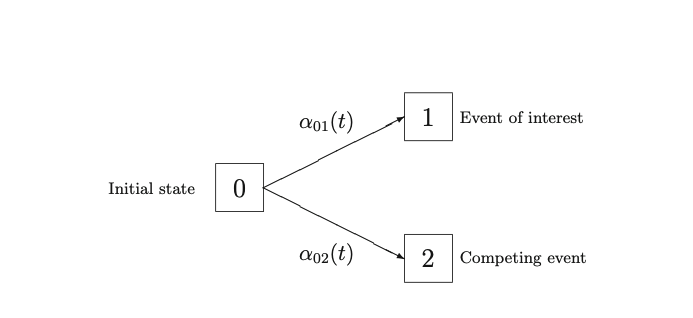
\includegraphics[width=1\linewidth]{Imagen1}

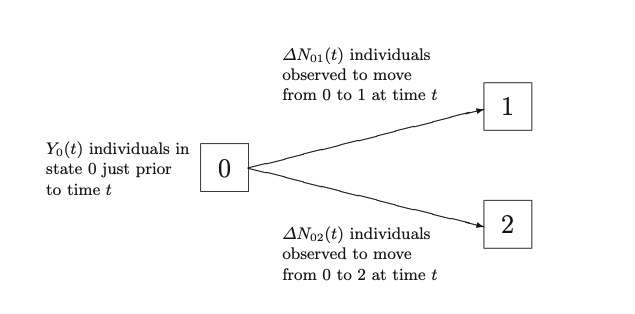
\includegraphics[width=1\linewidth]{Imagen_2}

Lo hacemos definiendo una matriz de valores lógicos inficando los
posibles tipos de transición en nuestro modelo multiestado:

\begin{Shaded}
\begin{Highlighting}[]
\NormalTok{tra }\OtherTok{\textless{}{-}} \FunctionTok{matrix}\NormalTok{(}\ConstantTok{FALSE}\NormalTok{, }\AttributeTok{ncol =} \DecValTok{3}\NormalTok{, }\AttributeTok{nrow =} \DecValTok{3}\NormalTok{)}
\FunctionTok{dimnames}\NormalTok{(tra) }\OtherTok{\textless{}{-}} \FunctionTok{list}\NormalTok{(}\FunctionTok{c}\NormalTok{(}\StringTok{"0"}\NormalTok{, }\StringTok{"1"}\NormalTok{, }\StringTok{"2"}\NormalTok{), }\FunctionTok{c}\NormalTok{(}\StringTok{"0"}\NormalTok{, }\StringTok{"1"}\NormalTok{, }\StringTok{"2"}\NormalTok{))  }
\NormalTok{tra[}\DecValTok{1}\NormalTok{, }\DecValTok{2}\SpecialCharTok{:}\DecValTok{3}\NormalTok{] }\OtherTok{\textless{}{-}} \ConstantTok{TRUE}
\NormalTok{tra}
\end{Highlighting}
\end{Shaded}

\begin{verbatim}
##       0     1     2
## 0 FALSE  TRUE  TRUE
## 1 FALSE FALSE FALSE
## 2 FALSE FALSE FALSE
\end{verbatim}

Esta matriz nos dice que un individup se puede mover del estado 0 al
estado 1, y del estado 0 al estado 2, pero las transiciones en el
sentido contrario no son posibles; además los valores en diagonal están
como falsos: Las transiciones de un estado a sí mismo no están
modeladas. No es necesario un modelo para dicha ``transición''. Los
individuos que no hacen una transición a uno de los dos pares
competitivos al tiempo t, permanece en el estado inicial 0 a tiempo t.

Ahora, calculamos la función de acumulación de riesgos específicos para
muerte y dados de alta, respectivamente, y estratificados por su estatus
de neumonía al momento de admisión:

\begin{Shaded}
\begin{Highlighting}[]
\DocumentationTok{\#\# sin neumonía }
\NormalTok{my.nelaal.nop }\OtherTok{\textless{}{-}} \FunctionTok{mvna}\NormalTok{(my.sir.data[my.sir.data}\SpecialCharTok{$}\NormalTok{pneu }\SpecialCharTok{==} \DecValTok{0}\NormalTok{, ], }\FunctionTok{c}\NormalTok{(}\StringTok{"0"}\NormalTok{, }\StringTok{"1"}\NormalTok{, }\StringTok{"2"}\NormalTok{), tra, }\StringTok{"cens"}\NormalTok{) }
\DocumentationTok{\#\# con neumonía}
\NormalTok{my.nelaal.p }\OtherTok{\textless{}{-}} \FunctionTok{mvna}\NormalTok{(my.sir.data[my.sir.data}\SpecialCharTok{$}\NormalTok{pneu }\SpecialCharTok{==} \DecValTok{1}\NormalTok{, ], }\FunctionTok{c}\NormalTok{(}\StringTok{"0"}\NormalTok{, }\StringTok{"1"}\NormalTok{, }\StringTok{"2"}\NormalTok{), tra, }\StringTok{"cens"}\NormalTok{)}
\end{Highlighting}
\end{Shaded}

Graficamos:

\begin{Shaded}
\begin{Highlighting}[]
\CommentTok{\# Estilo de la gráfica}
\NormalTok{ltheme }\OtherTok{\textless{}{-}} \FunctionTok{canonical.theme}\NormalTok{(}\AttributeTok{color =} \ConstantTok{FALSE}\NormalTok{) }
\NormalTok{ltheme}\SpecialCharTok{$}\NormalTok{strip.background}\SpecialCharTok{$}\NormalTok{col }\OtherTok{\textless{}{-}} \StringTok{"white"} 
\FunctionTok{lattice.options}\NormalTok{(}\AttributeTok{default.theme =}\NormalTok{ ltheme)}
\end{Highlighting}
\end{Shaded}

\begin{Shaded}
\begin{Highlighting}[]
\CommentTok{\#Plot para los que no tenían neumonía}
\NormalTok{dessin.nop }\OtherTok{\textless{}{-}} \FunctionTok{xyplot}\NormalTok{(my.nelaal.nop, }\AttributeTok{tr.choice =} \FunctionTok{c}\NormalTok{(}\StringTok{"0 2"}\NormalTok{, }\StringTok{"0 1"}\NormalTok{), }\AttributeTok{lwd =} \DecValTok{2}\NormalTok{, }\AttributeTok{layout =} \FunctionTok{c}\NormalTok{(}\DecValTok{1}\NormalTok{, }\DecValTok{2}\NormalTok{), }\AttributeTok{strip =} \FunctionTok{strip.custom}\NormalTok{( }\AttributeTok{factor.levels =} \FunctionTok{c}\NormalTok{(}\StringTok{"Sin neumonía:recuperación"}\NormalTok{, }\StringTok{"Sin Neumonía: Muertos"}\NormalTok{), }\AttributeTok{par.strip.text =} \FunctionTok{list}\NormalTok{(}\AttributeTok{font =} \DecValTok{2}\NormalTok{)), }\AttributeTok{ylim =} \FunctionTok{c}\NormalTok{(}\DecValTok{0}\NormalTok{, }\DecValTok{9}\NormalTok{), }\AttributeTok{xlim =} \FunctionTok{c}\NormalTok{(}\DecValTok{0}\NormalTok{, }\DecValTok{190}\NormalTok{), }\AttributeTok{xlab =} \StringTok{"Days"}\NormalTok{, }\AttributeTok{scales =} \FunctionTok{list}\NormalTok{(}\AttributeTok{alternating =} \DecValTok{1}\NormalTok{, }\AttributeTok{x =} \FunctionTok{list}\NormalTok{(}\AttributeTok{at =} \FunctionTok{seq}\NormalTok{(}\DecValTok{0}\NormalTok{, }\DecValTok{150}\NormalTok{, }\DecValTok{50}\NormalTok{)), }\AttributeTok{y =} \FunctionTok{list}\NormalTok{(}\AttributeTok{at =} \FunctionTok{seq}\NormalTok{(}\DecValTok{0}\NormalTok{, }\DecValTok{8}\NormalTok{, }\DecValTok{2}\NormalTok{))))}
\end{Highlighting}
\end{Shaded}

\begin{Shaded}
\begin{Highlighting}[]
\CommentTok{\#Plot para los que tenían neumonía}
\NormalTok{dessin.p }\OtherTok{\textless{}{-}} \FunctionTok{xyplot}\NormalTok{(my.nelaal.p, }\AttributeTok{tr.choice =} \FunctionTok{c}\NormalTok{(}\StringTok{"0 2"}\NormalTok{, }\StringTok{"0 1"}\NormalTok{), }\AttributeTok{lwd =} \DecValTok{2}\NormalTok{, }\AttributeTok{layout =} \FunctionTok{c}\NormalTok{(}\DecValTok{1}\NormalTok{, }\DecValTok{2}\NormalTok{), }\AttributeTok{strip =} \FunctionTok{strip.custom}\NormalTok{( }\AttributeTok{factor.levels =} \FunctionTok{c}\NormalTok{(}\StringTok{"Con neumonía:recuperación"}\NormalTok{, }\StringTok{"Con neumonía: Muertos"}\NormalTok{), }\AttributeTok{par.strip.text =} \FunctionTok{list}\NormalTok{(}\AttributeTok{font =} \DecValTok{2}\NormalTok{)), }\AttributeTok{ylab =} \StringTok{""}\NormalTok{, }\AttributeTok{ylim =} \FunctionTok{c}\NormalTok{(}\DecValTok{0}\NormalTok{, }\DecValTok{9}\NormalTok{), }\AttributeTok{xlim =} \FunctionTok{c}\NormalTok{(}\DecValTok{0}\NormalTok{, }\DecValTok{190}\NormalTok{), }\AttributeTok{xlab =} \StringTok{"Days"}\NormalTok{, }\AttributeTok{scales =} \FunctionTok{list}\NormalTok{(}\AttributeTok{alternating =} \DecValTok{1}\NormalTok{, }\AttributeTok{x =} \FunctionTok{list}\NormalTok{(}\AttributeTok{at =} \FunctionTok{seq}\NormalTok{(}\DecValTok{0}\NormalTok{, }\DecValTok{150}\NormalTok{, }\DecValTok{50}\NormalTok{)), }\AttributeTok{y =} \FunctionTok{list}\NormalTok{(}\AttributeTok{at =} \FunctionTok{seq}\NormalTok{(}\DecValTok{0}\NormalTok{, }\DecValTok{8}\NormalTok{, }\DecValTok{2}\NormalTok{))))}
\end{Highlighting}
\end{Shaded}

\begin{Shaded}
\begin{Highlighting}[]
\CommentTok{\#Ploteamos ambas}
\FunctionTok{print}\NormalTok{(dessin.nop, }\AttributeTok{split =} \FunctionTok{c}\NormalTok{(}\DecValTok{1}\NormalTok{, }\DecValTok{1}\NormalTok{, }\DecValTok{2}\NormalTok{, }\DecValTok{1}\NormalTok{), }\AttributeTok{more =} \ConstantTok{TRUE}\NormalTok{, }\AttributeTok{position =} \FunctionTok{c}\NormalTok{(}\DecValTok{0}\NormalTok{, }\DecValTok{0}\NormalTok{, }\FloatTok{1.07}\NormalTok{, }\DecValTok{1}\NormalTok{)) }
\FunctionTok{print}\NormalTok{(dessin.p, }\AttributeTok{split =} \FunctionTok{c}\NormalTok{(}\DecValTok{2}\NormalTok{, }\DecValTok{1}\NormalTok{, }\DecValTok{2}\NormalTok{, }\DecValTok{1}\NormalTok{), }\AttributeTok{position =} \FunctionTok{c}\NormalTok{(}\SpecialCharTok{{-}}\FloatTok{0.07}\NormalTok{, }\DecValTok{0}\NormalTok{, }\DecValTok{1}\NormalTok{, }\DecValTok{1}\NormalTok{))}
\end{Highlighting}
\end{Shaded}

\includegraphics{Proyecto_Riesgos_Competitivos_files/figure-latex/unnamed-chunk-19-1.pdf}

Esto no implica que la neumonía no tenga ningún efecto sobre la
mortalidad. La razón es que la neumonía parece reducir el riesgo de ser
dados de alta Esto implica:

\begin{enumerate}
\def\labelenumi{\arabic{enumi}.}
\item
  \begin{enumerate}
  \def\labelenumii{\arabic{enumii}.}
  \tightlist
  \item
    La neumonía parece reducir el riesgo por todas las causas al final
    de la de la unidad de cuidados intensivos.
  \end{enumerate}
\item
  Los pacientes con neumonía al ingreso permanecen más tiempo en la
  unidad. Durante esta estancia prolongada, están expuestos a un a un
  riesgo de muerte esencialmente
\item
  En consecuencia, mueren más pacientes con neumonía que sin neumonía.
\end{enumerate}

Se trata de un fenómeno típico de riesgos competitivos. Como hay más de
un riesgo que actúan sobre un individuo, no podemos saber, a partir de
un solo riesgo, cuál será el curso futuro de un individuo. Esta
situación se muestra de forma esquemática en la siguiente figura:

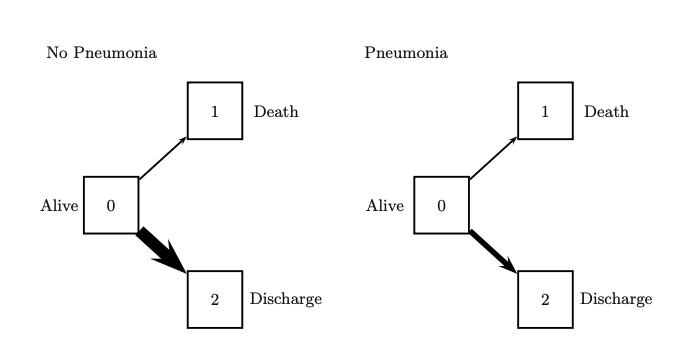
\includegraphics[width=1\linewidth]{pic_1} Fig. 1: Datos del hospital.
Representación esquemática del efecto de la neumonía con causa
específica. El estado de la neumonía no tiene ningún efecto sobre la
causa específica de muerte, que es también un peligro menor. Un gráfico
como el presente podían producirse con el paquete R compeir; hasta antes
de ser deshabilitada del CRAN

Recordemos que una forma de pensar en los peligros de causas específicas
es en términos de fuerzas momentáneas de transición que se mueven a lo
largo de las flechas de los cuadros multiestado. La magnitud de estas
fuerzas se muestra de forma esquemática en la figura 1. La ``fuerza de
muerte'' no está influenciada por el estado de la neumonía, pero la
``fuerza del alta'' se reduce sustancialmente de la neumonía en el
momento del ingreso. La figura 1 ilustra que la ``fuerza global'', es
decir, el riesgo por todas las causas que arrastra un individuo se ve
reducido, conduciendo a una mayor permanencia en la unidad, y que la
fuerza relativa entre las fuerzas específicas de la causa de muerte y de
alta, se ve modificada por el estado de la neumonía.

Notemos que la representación esquemática de la figura 1 tiene
limitaciones. La magnitud de las fuerzas de transición momentánea no
suele ser constante sobre el tiempo, de modo que necesitaríamos toda una
serie de gráficos como los de la figura 1. De hecho, esto se consigue en
la gráfica que ploteamos anteriormente de los estimadores de
Nelson-Aalen; la forma de los estimadores de dichos estimadores, que
estiman los peligros acumulativos, está determinada por los peligros
específicos de la causa. También podemos pensar en la figura 1 de una
manera que no necesariamente ilustre la magnitud de los peligros,
pudiendo variar con el tiempo, sino únicamente los cocientes de los
peligros de muerte y los cocientes de los peligros de descarga,
respectivamente, suponiendose constantes. Este es el enfoque adoptado
por la modelización de los riesgos proporcionales a la causa.

\hypertarget{funciuxf3n-de-incidencia-acumulada}{%
\subsection{Función de incidencia
acumulada}\label{funciuxf3n-de-incidencia-acumulada}}

Por último, comprobamos si nuestra interpretación del análisis de
riesgos acumulativos ha sido correcta observando los estimadores de
Aalen-Johansen de las funciones de incidencia acumulada, nuevamente
estratificadas por el estado de la neumonía. Recordemos que la función
de incidencia acumulada para la muerte, por ejemplo, muestra la
proporción esperada de individuos que mueren en la unidad a lo largo del
tiempo. Si nuestra interpretación del análisis de riesgos acumulativos
ha sido correcta, la función de incidencia acumulativa estimada para la
muerte\ldots\ldots. dentro de los pacientes con neumonía, debería estar
por encima de los pacientes sin neumonía.

Utilizando la función cuminc del paquete cmprsk, calculamos las
estimaciones \(\mathbb{P}( T \leq t, X_{T} = j), j = 1, 2\) (Es decir,
de la función acumulativa de incidencia) dentro de los grupos definidos

\begin{Shaded}
\begin{Highlighting}[]
\NormalTok{my.sir.cif }\OtherTok{\textless{}{-}} \FunctionTok{cuminc}\NormalTok{(my.sir.data}\SpecialCharTok{$}\NormalTok{time, my.sir.data}\SpecialCharTok{$}\NormalTok{to, }\AttributeTok{group=}\NormalTok{my.sir.data}\SpecialCharTok{$}\NormalTok{pneu, }\AttributeTok{cencode=}\StringTok{"cens"}\NormalTok{)}
\NormalTok{my.sir.cif}
\end{Highlighting}
\end{Shaded}

\begin{verbatim}
## Tests:
##       stat           pv df
## 1 16.16525 5.804939e-05  1
## 2 42.07480 8.784784e-11  1
## Estimates and Variances:
## $est
##             50        100        150
## 0 1 0.07930062 0.08576614 0.08576614
## 1 1 0.18393349 0.22550113         NA
## 0 2 0.88998816 0.91100110 0.91261748
## 1 2 0.64633198 0.73293123         NA
## 
## $var
##               50          100          150
## 0 1 0.0001125301 0.0001222882 0.0001222882
## 1 1 0.0016495598 0.0020723886           NA
## 0 2 0.0001517978 0.0001266104 0.0001250158
## 1 2 0.0025299050 0.0022581560           NA
\end{verbatim}

El valor regresado por cuminc es una lista con los componentes ``0 1'',
``1 1'', ``0 2'' y ``1 2''. Los componentes ``0 1'' y ``1 1'' contienen
resultados para el tipo de fallo 1; los componentes ``0 2'' y ``1 2''
contienen resultados para el tipo de fallo 2. Los componentes Los
componentes ``0 1'' y ``0 2'' son para pacientes con estado de neumonía
0 al ingreso, es decir, sin neumonía, y los componentes ``1 1'' y ``1
2'' son para pacientes con estado de neumonía 1.

Esto también lo podemos hacer con la paquetería etm, para matrices de
transiciones; al igual que con mvna. Ejecutamos etm con cada estrato:

\begin{Shaded}
\begin{Highlighting}[]
\NormalTok{my.sir.etm.nop }\OtherTok{\textless{}{-}} \FunctionTok{etm}\NormalTok{(my.sir.data[my.sir.data}\SpecialCharTok{$}\NormalTok{pneu }\SpecialCharTok{==} \DecValTok{0}\NormalTok{, ], }\FunctionTok{c}\NormalTok{(}\StringTok{"0"}\NormalTok{, }\StringTok{"1"}\NormalTok{, }\StringTok{"2"}\NormalTok{), tra, }\StringTok{"cens"}\NormalTok{, }\AttributeTok{s =} \DecValTok{0}\NormalTok{) }
\NormalTok{my.sir.etm.p }\OtherTok{\textless{}{-}} \FunctionTok{etm}\NormalTok{(my.sir.data[my.sir.data}\SpecialCharTok{$}\NormalTok{pneu }\SpecialCharTok{==} \DecValTok{1}\NormalTok{, ], }\FunctionTok{c}\NormalTok{(}\StringTok{"0"}\NormalTok{, }\StringTok{"1"}\NormalTok{, }\StringTok{"2"}\NormalTok{), tra, }\StringTok{"cens"}\NormalTok{, }\AttributeTok{s =} \DecValTok{0}\NormalTok{)}
\end{Highlighting}
\end{Shaded}

Graficando:

\begin{Shaded}
\begin{Highlighting}[]
\NormalTok{op }\OtherTok{\textless{}{-}} \FunctionTok{par}\NormalTok{(}\AttributeTok{mfrow =} \FunctionTok{c}\NormalTok{(}\DecValTok{1}\NormalTok{, }\DecValTok{2}\NormalTok{)) }
\CommentTok{\#Muerte }
\FunctionTok{plot}\NormalTok{(my.sir.etm.nop, }\AttributeTok{tr.choice =} \StringTok{"0 1"}\NormalTok{, }\AttributeTok{conf.int =} \ConstantTok{FALSE}\NormalTok{, }\AttributeTok{lwd =} \DecValTok{2}\NormalTok{, }\AttributeTok{lty =} \DecValTok{1}\NormalTok{, }\AttributeTok{xlab =} \StringTok{"Días"}\NormalTok{, }\AttributeTok{ylab =} \StringTok{"Probabilidad"}\NormalTok{, }\AttributeTok{bty =} \StringTok{"n"}\NormalTok{, }\AttributeTok{legend =} \ConstantTok{FALSE}\NormalTok{)}
\FunctionTok{lines}\NormalTok{(my.sir.etm.p, }\AttributeTok{tr.choice =} \StringTok{"0 1"}\NormalTok{, }\AttributeTok{conf.int =} \ConstantTok{FALSE}\NormalTok{, }\AttributeTok{lwd =} \DecValTok{2}\NormalTok{, }\AttributeTok{lty =} \DecValTok{2}\NormalTok{)}
\FunctionTok{legend}\NormalTok{(}\DecValTok{0}\NormalTok{, }\FloatTok{0.6}\NormalTok{, }\FunctionTok{c}\NormalTok{(}\StringTok{"neumonía"}\NormalTok{, }\StringTok{"sin neumonía"}\NormalTok{), }\AttributeTok{col =} \DecValTok{1}\NormalTok{, }\AttributeTok{lty =} \FunctionTok{c}\NormalTok{(}\DecValTok{1}\NormalTok{, }\DecValTok{2}\NormalTok{), }\AttributeTok{bty =} \StringTok{"n"}\NormalTok{, }\AttributeTok{lwd =} \DecValTok{2}\NormalTok{) }
\FunctionTok{title}\NormalTok{(}\StringTok{"Muerte"}\NormalTok{) }
\FunctionTok{axis}\NormalTok{(}\DecValTok{1}\NormalTok{, }\AttributeTok{at =} \FunctionTok{seq}\NormalTok{(}\DecValTok{0}\NormalTok{, }\DecValTok{200}\NormalTok{, }\DecValTok{50}\NormalTok{)) }
\DocumentationTok{\#\#Dados de alta }
\FunctionTok{plot}\NormalTok{(my.sir.etm.nop, }\AttributeTok{tr.choice =} \StringTok{"0 2"}\NormalTok{, }\AttributeTok{conf.int =} \ConstantTok{FALSE}\NormalTok{, }\AttributeTok{lwd =} \DecValTok{2}\NormalTok{, }\AttributeTok{lty =} \DecValTok{1}\NormalTok{, }\AttributeTok{xlab =} \StringTok{"Días"}\NormalTok{, }\AttributeTok{ylab =} \StringTok{"Probabilidad"}\NormalTok{, }\AttributeTok{bty =} \StringTok{"n"}\NormalTok{, }\AttributeTok{legend =} \ConstantTok{FALSE}\NormalTok{)}
\FunctionTok{lines}\NormalTok{(my.sir.etm.p, }\AttributeTok{tr.choice =} \StringTok{"0 2"}\NormalTok{, }\AttributeTok{conf.int =} \ConstantTok{FALSE}\NormalTok{, }\AttributeTok{lwd =} \DecValTok{2}\NormalTok{, }\AttributeTok{lty =} \DecValTok{2}\NormalTok{) }
\FunctionTok{axis}\NormalTok{(}\DecValTok{1}\NormalTok{, }\AttributeTok{at =} \FunctionTok{seq}\NormalTok{(}\DecValTok{0}\NormalTok{, }\DecValTok{200}\NormalTok{, }\DecValTok{50}\NormalTok{)) }
\FunctionTok{title}\NormalTok{(}\StringTok{"Recuperados"}\NormalTok{) }
\end{Highlighting}
\end{Shaded}

\includegraphics{Proyecto_Riesgos_Competitivos_files/figure-latex/unnamed-chunk-22-1.pdf}

\begin{Shaded}
\begin{Highlighting}[]
\FunctionTok{par}\NormalTok{(op)}
\end{Highlighting}
\end{Shaded}

Esta gráfica presenta las estimaciones de Aalen-Johansen
\(\mathbb{P}( b T ≤ t, X_{T} = j)\) de las funciones de incidencia
acumulativa para la muerte (izquierda, j = 1) y para el alta (derecha, j
= 2), estratificadas por el estado de la neumonía al ingreso. Las líneas
continuas corresponden a pacientes sin neumonía.

Como era de esperarse, encontramos que mueren más pacientes entre los
que tienen neumonía.

Las estimaciones de Aalen-Johansen \(\mathbb{P}( T ≤ t, X_{T} = 1)\) se
muestran en la siguiente gráfica, junto con intervalos de confianza del
95\% puntuales, generadas por:

\begin{Shaded}
\begin{Highlighting}[]
\FunctionTok{plot}\NormalTok{(my.sir.etm.p, }\AttributeTok{tr.choice =} \StringTok{\textquotesingle{}0 1\textquotesingle{}}\NormalTok{, }\AttributeTok{col =} \DecValTok{1}\NormalTok{, }\AttributeTok{lwd =} \DecValTok{2}\NormalTok{, }\AttributeTok{conf.int =} \ConstantTok{TRUE}\NormalTok{, }\AttributeTok{ci.fun =} \StringTok{"cloglog"}\NormalTok{, }\AttributeTok{legend =} \ConstantTok{FALSE}\NormalTok{, }\AttributeTok{ylab=}\StringTok{"Probability"}\NormalTok{, }\AttributeTok{xlim=}\FunctionTok{c}\NormalTok{(}\DecValTok{0}\NormalTok{,}\DecValTok{190}\NormalTok{))}
\FunctionTok{lines}\NormalTok{(my.sir.etm.nop, }\AttributeTok{tr.choice =} \StringTok{\textquotesingle{}0 1\textquotesingle{}}\NormalTok{, }\AttributeTok{col =} \StringTok{"gray"}\NormalTok{, }\AttributeTok{lwd =} \DecValTok{2}\NormalTok{, }\AttributeTok{conf.int =} \ConstantTok{TRUE}\NormalTok{, }\AttributeTok{ci.fun =} \StringTok{"cloglog"}\NormalTok{)}
\FunctionTok{legend}\NormalTok{(}\DecValTok{0}\NormalTok{, }\DecValTok{1}\NormalTok{, }\FunctionTok{c}\NormalTok{(}\StringTok{"neumonía"}\NormalTok{, }\StringTok{"sin neumonía"}\NormalTok{), }\AttributeTok{col =} \DecValTok{1}\NormalTok{, }\AttributeTok{lty =} \FunctionTok{c}\NormalTok{(}\DecValTok{1}\NormalTok{, }\DecValTok{2}\NormalTok{), }\AttributeTok{bty =} \StringTok{"n"}\NormalTok{, }\AttributeTok{lwd =} \DecValTok{2}\NormalTok{)}
\FunctionTok{title}\NormalTok{(}\StringTok{"Estimador Aalen{-}Johansen con intervalos de confianza"}\NormalTok{)}
\end{Highlighting}
\end{Shaded}

\includegraphics{Proyecto_Riesgos_Competitivos_files/figure-latex/unnamed-chunk-23-1.pdf}

Los intervalos de confianza apoyan nuestra conclusión anterior de que
finalmente vemos más casos de muerte en el grupo de pacientes con
neumonía. Los gráficos de riesgos acumulados, como en la fgráfica de
riesgos acumulados (La primera gráfica presentada), y los gráficos de
funciones de incidencia acumulada, como en las Figuras 2 y 3, ambos
tienen sus méritos relativos: Obviamente, en la figura 3 es más fácil
saber si la neumonía aumenta la mortalidad unitaria. Sin embargo,
tenemos que examinar los peligros acumulados por causas específicas para
ver si el aumento de la mortalidad se debe a un aumento del peligro de
muerte, o, como en el presente ejemplo, a una disminución del riesgo de
muerte.

\end{document}
